\documentclass[12pt]{article}
\usepackage[english]{babel}
% \usepackage[utf8x]{inputenc}
\usepackage[T1]{fontenc}
\usepackage{scribe}
\usepackage{listings}
\usepackage{fullpage}
\usepackage{amsfonts}
\usepackage{amssymb}
\usepackage{multirow}
\usepackage{multicol}
\usepackage{hyperref}
\usepackage{url}
\usepackage{subfig}
\usepackage[svgnames]{xcolor}
\usepackage{color}
\usepackage{hyperref}
\usepackage{parskip}
% \definecolor{light-gray}{gray}{0.90}
% \lstset{backgroundcolor=\color{light-gray},showlines=true}

% \usepackage{xcolor}
% \usepackage{listings}

% \lstdefinestyle{BashInputStyle}{
%   language=bash,
%   basicstyle=\small\sffamily,
%   numbers=left,
%   numberstyle=\tiny,
%   numbersep=3pt,
%   frame=tb,
%   columns=fullflexible,
%   backgroundcolor=\color{yellow!20},
%   linewidth=0.9\linewidth,
%   xleftmargin=0.1\linewidth
% }

\usepackage{minted}
\setminted{fontsize=\footnotesize,baselinestretch=0.5}

\Scribe{}
\Lecturer{Queenie Qiu, John Raiti. Student: \textbf{Shucheng Guo}}
\LectureNumber{4}
\LectureDate{DATE: Feb 2nd. 2023}
\LectureTitle{Safe wandering using path planning algorithms}

\lstset{style=mystyle}

\begin{document}
	\MakeScribeTop

\setlength{\parindent}{15pt}

%#############################################################
%#############################################################
%#############################################################
%#############################################################

\section{Learning Objectives}
\begin{enumerate}
    \item Review and modify code to execute different path planning algorithms on a simulated turtlebot3.
    
    \item Compare and contrast the performance of different algorithms (Djisktra and A*) as global planners in the ROS navigation stack.
    
    \item Explore challenges and limitations of different planning algorithms to learn the trade-offs of choosing one over another.
\end{enumerate}


\section{Install and test the global\_planner package}

This global\_planner package is one of the packages from the ros navigation stack meta-package. It provides a wrapper on the navigation class that allows to select the type of planning algorithm used for the global plan, using the information from a map. For this lab, we will assume the map has already been created and saved (.pgm and .yaml files). If you wish to try the global planner on a new environment, you can either launch the gmapping demo and save the new map, or add a gmapping node for SLAM in your launch file. Information about the 
\href{http://wiki.ros.org/nav_core}{navigation stack} and the \href{http://wiki.ros.org/global_planner}{global planner} can be found in the ROS wiki.

\begin{enumerate}
    \item Download the zip file with the global\_planner package from the course materials on canvas.
    \item Extract the zip file and place the global\_planner folder in your src folder in your workspace (~/catkin/src/). You will need to build your package from the /catkin\_ws/ directory. Make sure that all dependencies are installed before building the package:
    \begin{minted}{bash}
        $ rosdep install --from-paths src --ignore-src -r -y
    \end{minted}
    
    \begin{minted}{bash}
        $ catkin_make global_planner
    \end{minted}
    
    \item Once the build has successfully finished, source your new workspace (source devel/setup.bash), launch a turtlebot3 gazebo instance and run the test\_planner launch file:
    
    \begin{minted}{bash}
        $ roslaunch turtlebot3_gazebo turtlebot3_world.launch
    \end{minted}
    
    \begin{minted}{bash}
        $ roslaunch global_planner test_planner.launch
    \end{minted}
    
     You should be able to see the following topics as active after rostopic list:\\
        /move\_base/GlobalPlanner/plan\\
        /move\_base/GlobalPlanner/potential
    \item Once you find these topics in your list, your package is successfully installed. If you find any trouble with this, contact the instructors or TA.
\end{enumerate}

\section{Path planning algorithms}

\subsection{Adding the global planner to the turtlebot3 navigation stack.}
In previous labs, turtlebot3\_navigation.launch is launched before we used the 2D Nav Goal. If you look into the launch file, you will notice it launches move\_base.launch -- it is where to configure the planners in turtlebot's navigation stack. We want to create a new navigation stack by duplicating the launch files and modifying the copied files as needed.



% We will create similar content to the one used for the navigation example, including: the turtlebot3\_navigation.launch (in launch folder), move\_base.launch(in launch folder), and the .yaml parameters files (in the /param folder) in the turtlebot3\_navigation package.

\begin{enumerate}
    \item Make copies of launch files in the turtlebot3\_navigation package:
    \begin{enumerate}
        \item move\_base.launch → move\_base\_path\_planning.launch: the changes made to this new file are related with adding the global\_planner. Details will be provided later.
        \item turtlebot3\_navigation.launch → turtlebot3\_path\_planning.launch: the main difference in this new file is launching the move\_base\_path\_planning.launch file created in step a.
       
       You need to make the change in the "turtlebot3\_path\_planning.launch" file on the move\_base node to include the new move\_base\_path\_planning.launch file


    \end{enumerate}
    \item Download the parameters .yaml file (global\_planner\_params\_burger.yaml) and place it in the turtlebot3\_navigation/param folder. This file allows you to make changes to the global planner parameters. Refer to the \href{http://wiki.ros.org/global\_planner}{ROS wiki} for details on what each parameter does.
    
    \item In the move\_base\_path\_planning.launch file, add a global planner as a parameter of the move\_base node in the launch file:
    \begin{enumerate}
    \item <param name="base\_global\_planner" value="global\_planner/GlobalPlanner" />
    
    \item <rosparam file="\$(find turtlebot3\_navigation)/param/global\_planner\_params\_burger.yaml" command="load"/>

    \end{enumerate}
    \begin{figure}[H]
    \vspace{-10pt}
    \centering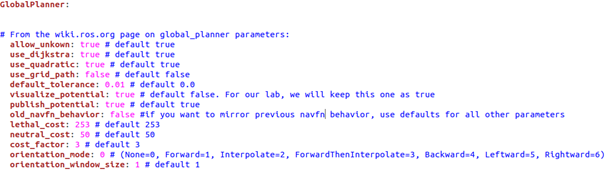
\includegraphics[width=14cm]{images/globalPlanner.png}\vspace{-10pt}
    \caption{Global Planner yaml file.}\label{fig:pid}
    \end{figure}
    
    \end{enumerate}

    \subsection{Run the new navigation stack.}
    \begin{enumerate}
    \item Launch a gazebo instance of the burger in the turtleworld3\_world:
    
     \begin{minted}{bash}
    $ roslaunch turtlebot3_gazebo turtlebot3_world.launch
    \end{minted}
    
    \item Launch the new turtlebot3\_path\_planning.launch. Before sending any Navigation goals, remember to provide a 2DEstimate for the actual position of the robot in RViz. For this lab, we will disable the Global and Local costmaps that come as default in the RViZ configuration for navigation.
     \begin{minted}{bash}
    $ roslaunch turtlebot3_navigation turtlebot3_path_planning.launch
    \end{minted}

    \textbf{Tip}: The 2DEstimate point with the RViz GUI provides the robot’s initial position and orientation; a large mismatch between the robot’s estimates and its actual position may result in a fatal error for the launched file.

    \item Customize the RViz visualization components
    \begin{enumerate}
        \item Turn off the Global Map and Local Map, and add by topic the GlobalPlanner/potential topic as another map. Choose costmap to be the color scheme.
        \item Change the topic of Planner Plan to GlobalPlanner/plan.
    \end{enumerate}
    
    \item Publish four sequential points for the robot to navigate towards($P_0 \rightarrow P_1\rightarrow P_2 \rightarrow P_3 \rightarrow P_0$). You may publish in the /move\_base/goal topic through a node (path\_planning\_goal.py from Canvas), or you may use rostopic pub from the command line. You will need to pay attention to the contents of the message as the pose is given by a position vector and an orientation using quaternions.

    \textbf{Notice}: The visualization of the potential map doesn't look like what the figure shows.
    
    \begin{figure}[H]
    \vspace{-10pt}
    \centering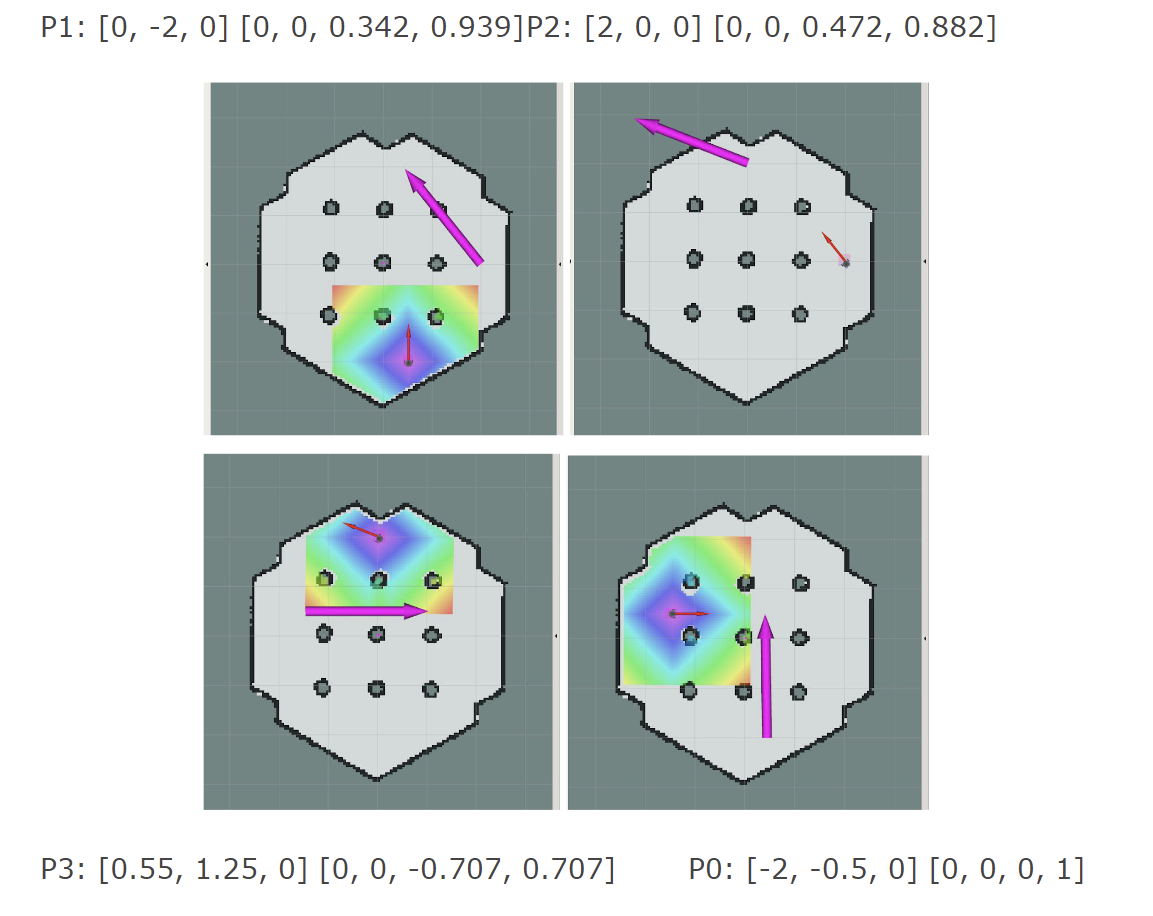
\includegraphics[width=10.3cm]{images/Fourpoints.png}\vspace{-10pt}
    \caption{Four sequential points.}\label{fig:sequential points}
    \end{figure}
    
    \item This sequence you will attempt using two global planners: Djikstra and A* (you will need to change the parameters accordingly and report your best performing combination)
    \begin{enumerate}
        \item As it will come to your attention, when using dijkstra the planner works best if you use gradient descent and not a grid; the opposite is true for A*. Also the value for neutral\_cost is relevant (lower for Dijkstra, medium for A*). The option of use\_quadratic may or may not help. The cost\_factor might influence how much the local planner will be used.
        
        \item Some parameters can be changed dynamically using the command:
        
        \begin{minted}{bash}
        $ rosrun rqt_reconfigure rqt_reconfigure
         \end{minted}

    \end{enumerate}
    
\end{enumerate}

\textbf{Deliverables:}

\begin{enumerate}
    \item For both global planners, you will also gather the following quantitative information (highly recommend to create a table):
    
    \begin{enumerate}
        
        \item For each chunk of the path ($P_0$ → $P_1$, $P_1$ → $P_2$, $P_2$ → $P_3$, $P_3$ → $P_0$), report the travel time (rough estimation is ok.)
        
        \textsc{Notice: }\\For Dijkstra algorithm, gradient descent was used for optimization.\\For A* algorithm, grid path was used, and \mintinline{bash}{neutral_cost} set to \mintinline{bash}{100}.
    
        \begin{table}[htb]
            \centering
            \begin{tabular}{|c|cc|}
            \hline
            \multirow{2}{*}{\textbf{Path}} & \multicolumn{2}{c|}{\textbf{Algorithm}}              \\ \cline{2-3} 
                                        & \multicolumn{1}{c|}{\textit{Dijkstra}} & \textit{A* Search} \\ \hline
            $P_0$ → $P_1$               & \multicolumn{1}{c|}{$23s$}                 & $27s$          \\ \hline
            $P_1$ → $P_2$               & \multicolumn{1}{c|}{$16s$}                 & $25s$          \\ \hline
            $P_2$ → $P_3$               & \multicolumn{1}{c|}{$22s$}                 & $26s$          \\ \hline
            $P_3$ → $P_0$               & \multicolumn{1}{c|}{$18s$}                 & $39s$          \\ \hline
            Total                       & \multicolumn{1}{c|}{$1m19s$}               & $1m57s$        \\ \hline
            \end{tabular}
            \end{table}
            \vspace{-5pt}
       
        \item Describe qualitatively whose path length was shorter for A* and Djikstra.
        
        \textbf{Answer: }The paths of the robot planned by both algorithms are demonstrated in Figure \ref{fig:odom_plot}. It's quite hard to tell just by eyes, which path is longer. Each algorithm performs differently depending on the condition, in accordance with their strategy. The A* path made detours in the first chunk, but walked in straighter lines in the next two.
        
        \item What did you observe from the potential map?
        
        \textbf{Answer: }The potentials of the path calculated by both algorithms are demonstrated in Figure \ref{fig:potentials}. It's obvious that the colored areas are larger along the path of the Dijkstra one than the A* one. It means that A* algorithm considers fewer potential paths, or only expands certain nodes closer to the goal, while Dijkstra explores in all directions.
       
        \item Discuss the advantages and disadvantages of the two path planning algorithm.
        
        \begin{multicols}{2}

            \textsc{Dijkstra}: a special case for A* without heuristics
            
            \textbf{Pros:}
            \begin{itemize}
                \item finds the optimal path by exploring all possibilities
                \item requires only source and goal node
                \item less memory usage
            \end{itemize}
            
            \textbf{Cons:}
            \begin{itemize}
                \item more operation time and resource consumption in general
                \item assumes a finite graph
                \item works only with non-negative edge costs or weights
            \end{itemize}

        \columnbreak
            \textsc{A* Search}: greedy best-first search with two cost functions
            
            \textbf{Pros:}
            \begin{itemize}
                \item achieves a trade-off between memory, time, and length
                \item explores the fewest number of nodes and paths
                \item less time complexity in theory
            \end{itemize}
            
            \textbf{Cons:}
            \begin{itemize}
                \item efficiency relies heavily on a good heuristic function
                \item finds optimal path only with admissible heuristic function
                \item more space complexity in theory
            \end{itemize}

        \end{multicols}
    
        \begin{figure}[h]
            \centering
            \subfloat[Dijkstra]{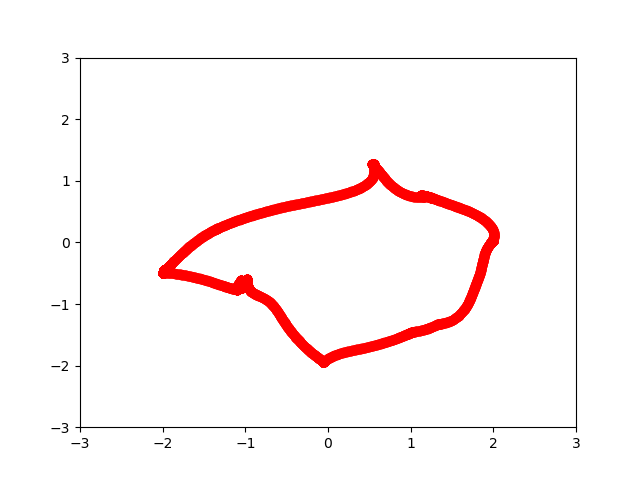
\includegraphics[width=.48\columnwidth]{images/odom_plot_dijkstra.png}}
            \subfloat[A* Search]{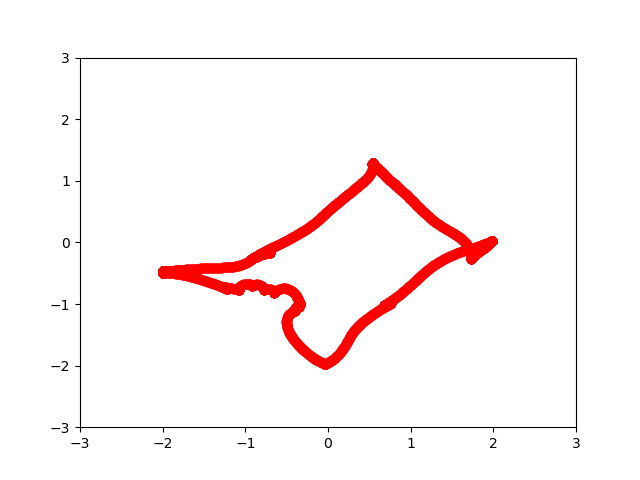
\includegraphics[width=.48\columnwidth]{images/odom_plot_a-star.png}}
            \caption{Plotting robot's paths planned by different algorithms.}
            \label{fig:odom_plot}
        \end{figure}

        \begin{figure}[h!]
            \centering
            \subfloat[Dijkstra]{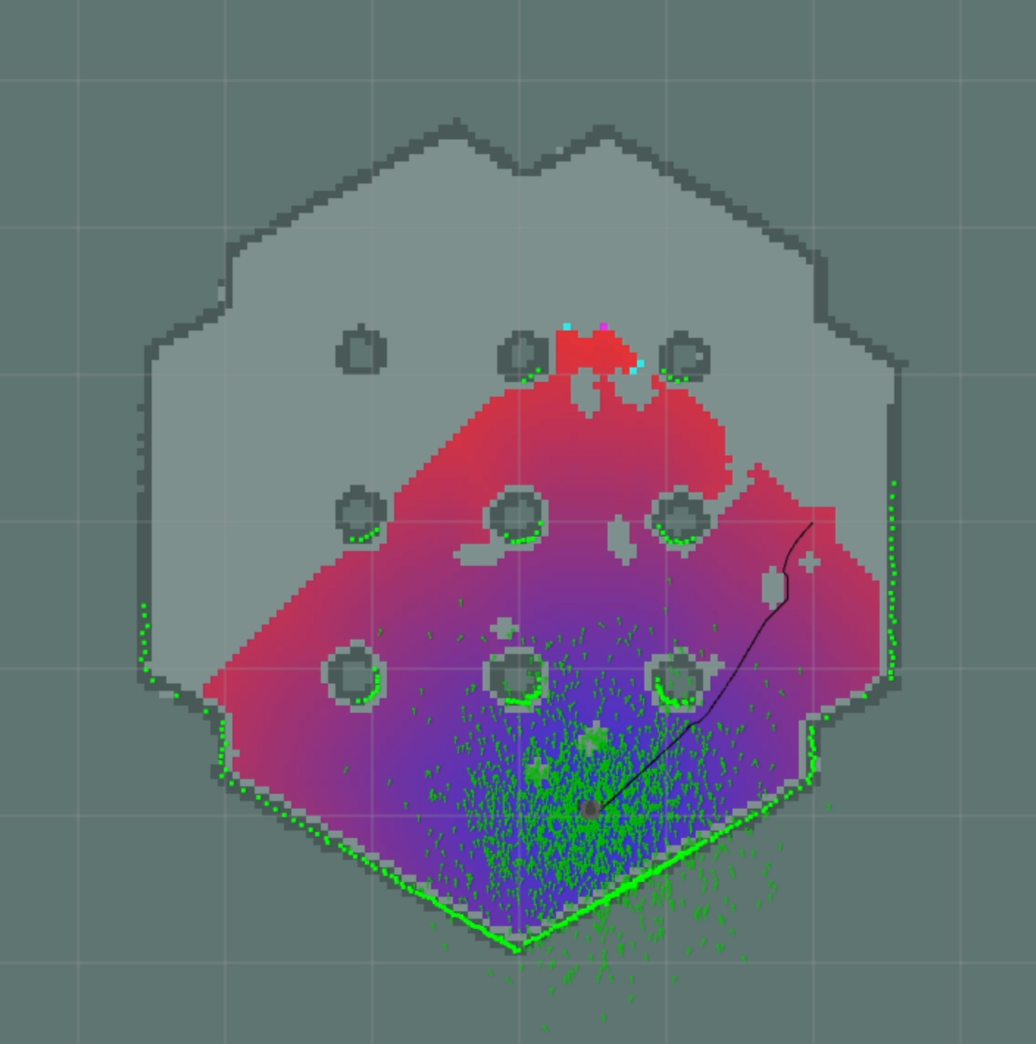
\includegraphics[width=.4\columnwidth]{images/costmap_dijkstra.png}}
            \hspace{3ex}
            \subfloat[A* Search]{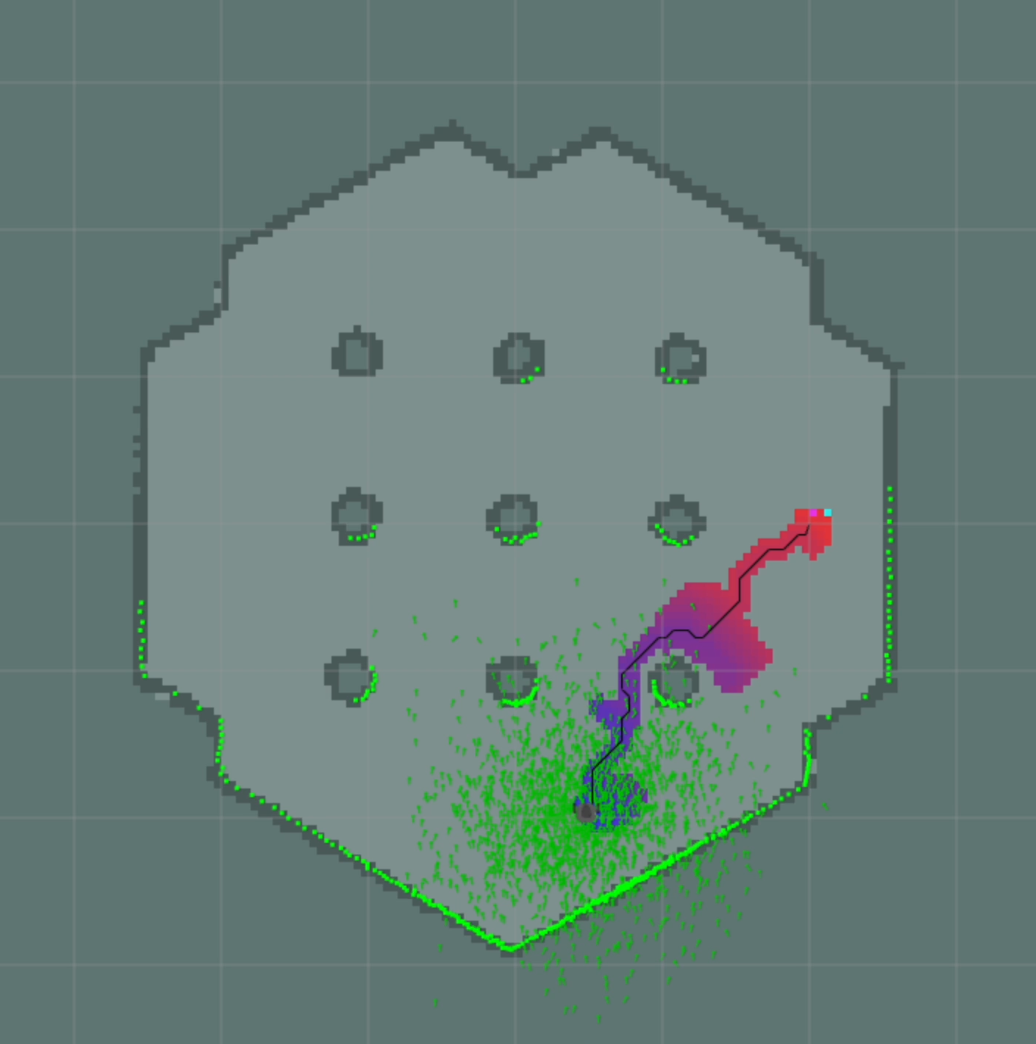
\includegraphics[width=.4\columnwidth]{images/costmap_a-star.png}}
            \caption{Calculating potentials by different algorithms.}
            \label{fig:potentials}
        \end{figure}

    \end{enumerate}
    
    \item Use your pillar model (created in Lab1), and add it as an obstacle in the turtlebot3\_world. Turn on the Local Map visualization in Rviz. Attempt to send a 2DNavigationGoal where the robot has to circumvent the new obstacle.
    \begin{enumerate}
        \item Report your choice for obstacle location by taking a screenshot, and your robot’s initial position as well as the selected goal position and orientation. (Tip: you may want to use the topic /move\_base/goal, and echo it, to obtain position and orientation vectors)
        
        \textbf{Answer: }The obstacle, a pillar of which the radius is $0.2m$, is placed right to $P_2$, at the point \mintinline{bash}{(1.68, -0.68, 0.25)}, as shown in Figure \ref{fig:obstacle}. The initial and goal nodes are set to $P_1$ and $P_2$ respectively for easier comparison. The obstacle is set such that it blocks the optimal path from $P_1$ to $P_2$ previously computed by the algorithm. It has to dynamically replan a new path that avoids the obstacle.
        \\$P_1$: \mintinline{bash}{(0, -2, 0)(0, 0, 0.342, 0.939)};\\$P_2$: \mintinline{bash}{(2, 0, 0)(0, 0, 0.472, 0.882)}.
        
        \begin{figure}[h]
            \centering
            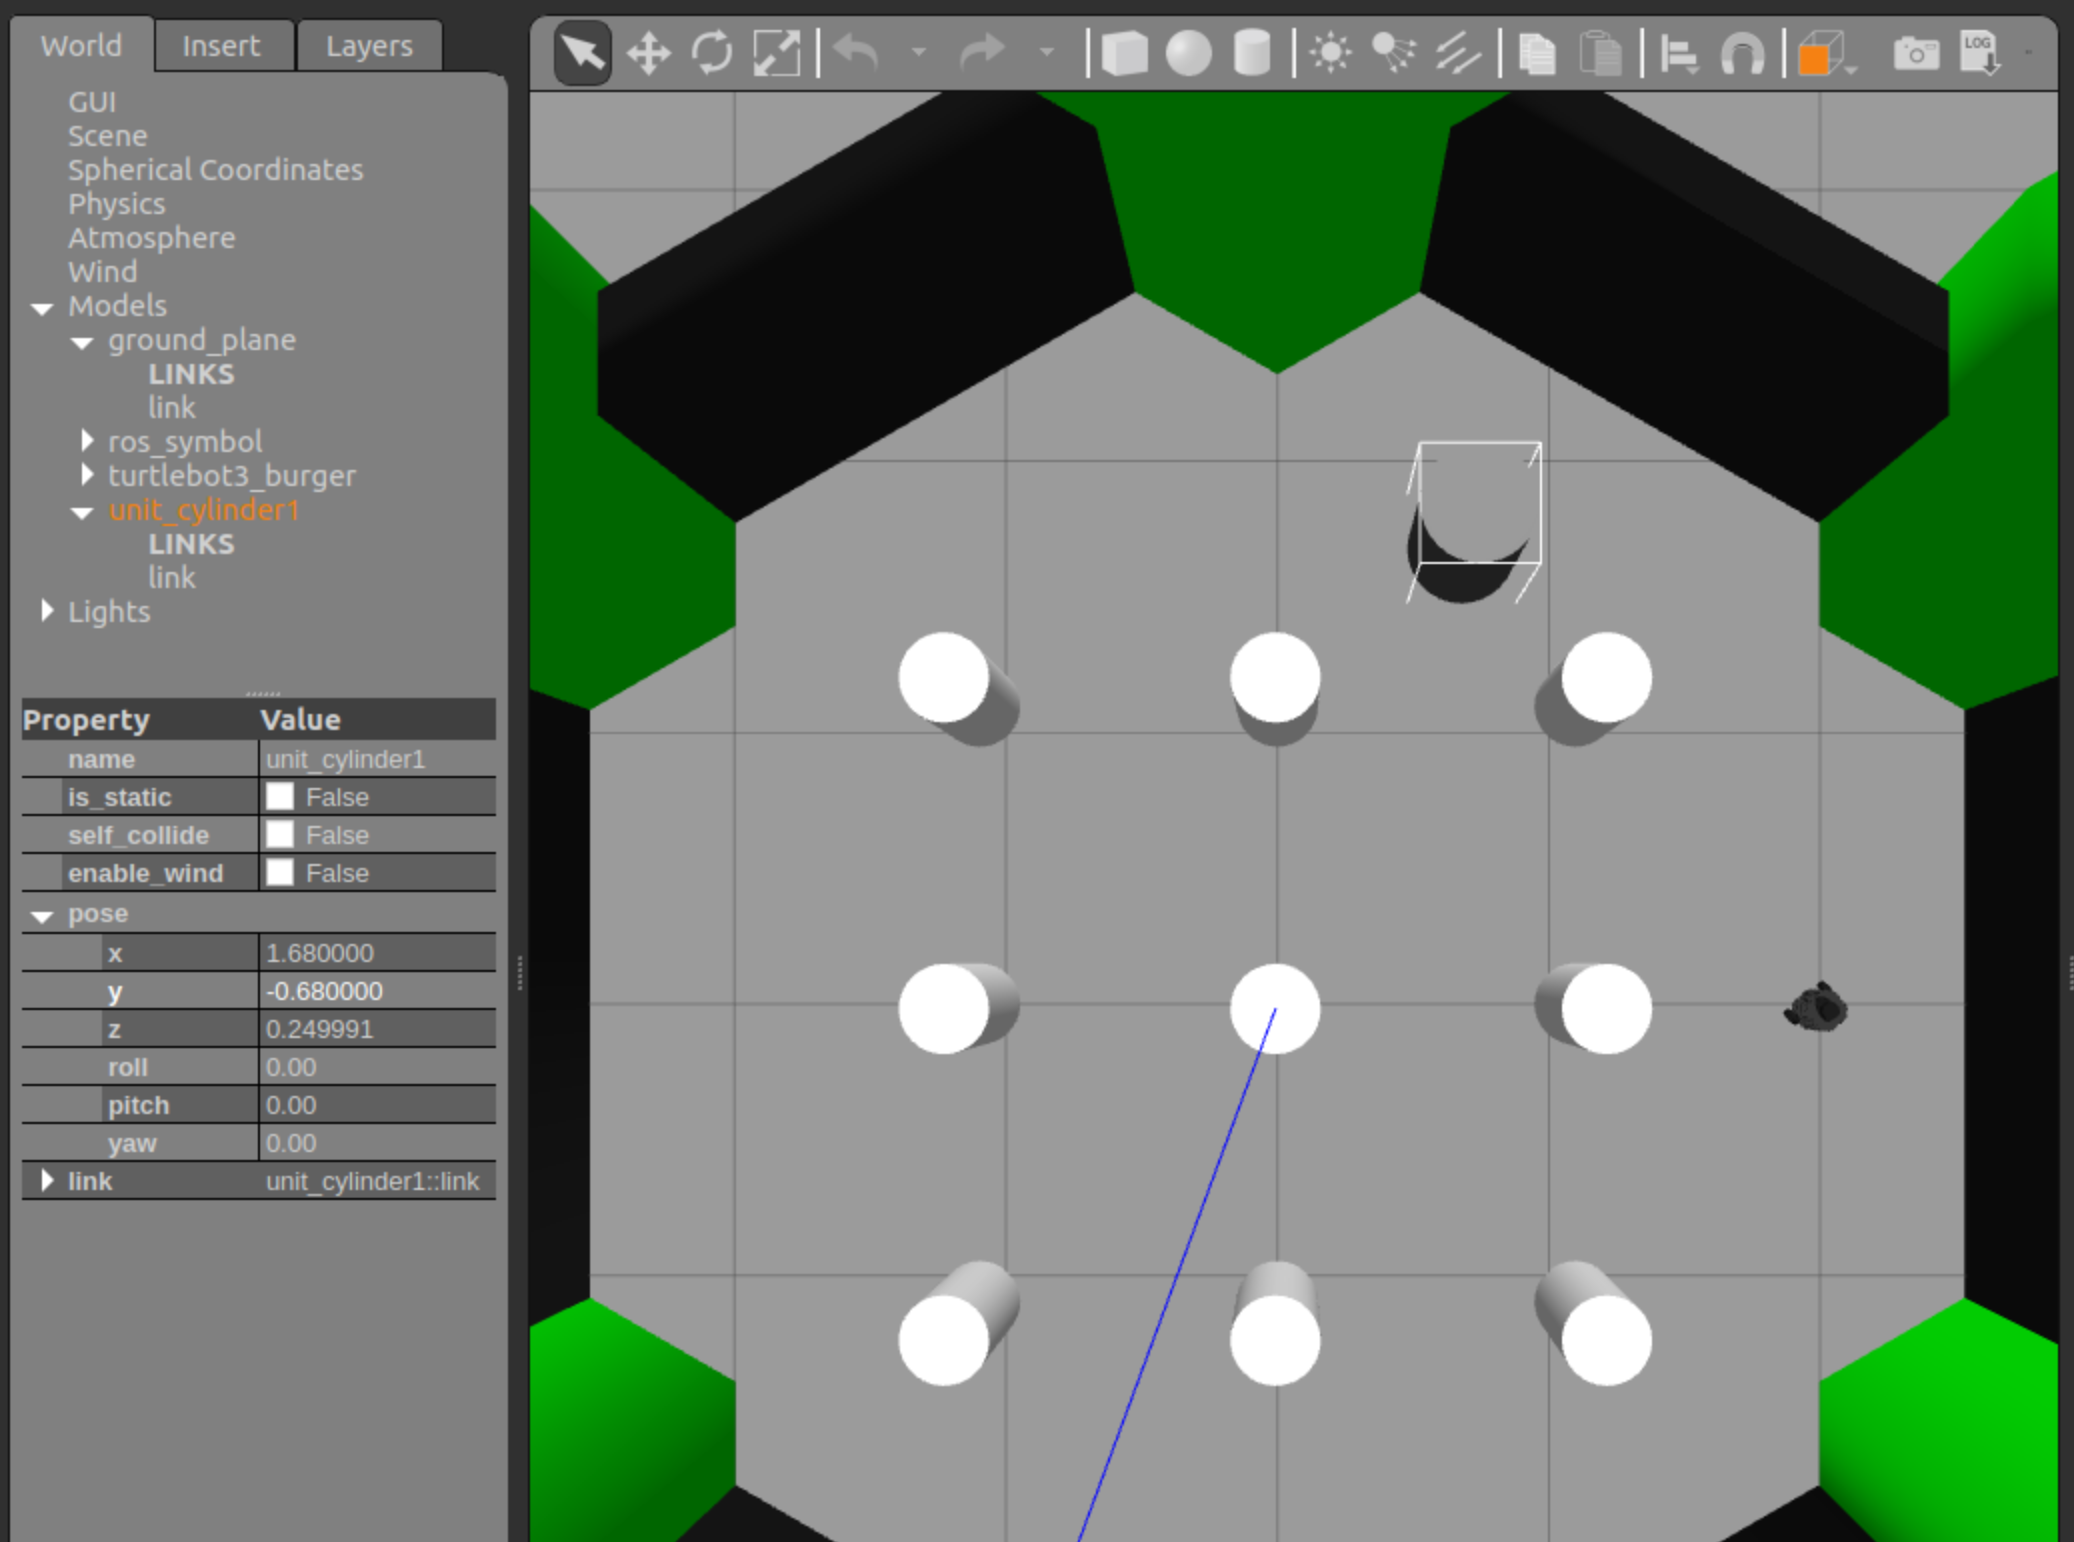
\includegraphics[width=10.3cm]{images/obstacle_pose.png}
            \caption{Position of pillar obstacle.}\label{fig:obstacle}
        \end{figure}
        
        \item Describe the actions of the robot: 
        
        \begin{enumerate}            
            \item Does the robot reach its intended goal in A* and Djikstra?
            
            \textbf{Answer: }For the aforementioned setting, in which the obstacle has a medium radius, the robot almost always reaches the goal. There were a few edge cases, where the robot was stuck in a narrow aisle between pillars.
            
            Doubling the radius of the obstacle, however, brings the success rate down to zero. With a larger pillar, the original path is completely blocked and a major retreat and detour is required. The robot under such algorithms is obviously not prepared.

            \item What did you observe from the global planner and local planner?
            
            \textbf{Answer: }The indicator for the global planner is a thin, black, and solid black line between the start and end nodes, while that for the local planner is a much shorter line in a lighter color that constantly changes.
            
            Although both indicators change, the local planner does it at a much faster speed. Based on their definition, it can be deducted that the global planner calculates the full path prior to operation and dynamically adjusts path during the process; the local planner generally follows the global planner, but modifies the full path if obstacles are detected along the way to prevent collisions.

            Specifically, the global planner subscribes to the map, current position, goal position, and publishes a path between both positions; the local planner subscribes to the map and the path planned by global planner, and publishes command velocities for the robot to best accomplish the goal. Should there be unexpected objects on the path not detected or considered by global planner, the local planner would dynamically adjust \mintinline{bash}{cmd_vel} for the robot to avoid them.

        \end{enumerate}
    \end{enumerate}
\end{enumerate}


\section{Path planning with the physical robot}

This portion of the lab assignment will entail repeating the same process for testing the two global planners, now using the GIX map. You have already completed a map for this environment. If you do not have the .pgm and .yaml files associated with the GIX map you will have to run the gmapping demo and teleoperate the robot around the map before getting started.

We will have to repeat the connection instructions for the physical robot. Changes to be made in the environment variables and the ~/.bashrc file.

Instead of providing a sequence of 4 points as navigation goals, the physical implementation will include only 2 points, with two paths: One from $P_0$ → $P_1$, and another $P_1$ → $P_0$. $P_0$ will be your starting position (marked with a black X), P1 will be marked by a blue X.

\textbf{Deliverables:}

    \begin{enumerate}
    \item Using the global\_planner with both algorithms (Dijkstra and A*) to report:
    
        \begin{enumerate}
            \item the travel time (rough estimation is ok.)
            
            \item If any collisions occur, note them and comment on possible causes of the collisions.
        \end{enumerate}
    
    \item Reset the robot to the initial position $P_0$, and then add an obstacle in the map environment. Attempt the navigation to $P_1$ and comment on the execution using both planners:
    
    \begin{enumerate}
        \item Does the robot reach its intended goal in A* and Djikstra?
        \item What did you observe from the global planner and local planner?

    \end{enumerate}

    \end{enumerate}



\end{document}